
\section{Arduino Variante}

In Abbildung \ref{fig-SchemaAufbau} ist der schematische Aufbau des Projektes zu sehen. Das Gießsystem besteht aus der Steuereinheit, dem Wasserbehälter sowie der Pumpe mit dem Schlauchsystem. Aus dem Steuergerät wird der Sensor über einen Chin"~Anschluss herausgeführt. Auf der linken Seite wird das Netzteil mit einem Hohlstecker verbunden. 
Im Folgenden beschreiben wir das Vorgehen für das Gießsystem basierend auf der Arduino Variante. 
Es wird hierzu auf folgende Bereiche eingegangen:

\begin{itemize}
	\item Zu Beginn beschreiben wir verschiedenen Möglichkeiten des Wassertransports zur Pflanze.
	\item Im weiteren stellen wir das Vorgehen zur Erstellung des Gehäuses für die Elektronik dar.
	\item In Abschnitt Elektronik werden wir auf den Aufbau der Platine und die hiermit verbunden Bereiche \emph{Sensorschaltung}, \emph{Stromversorgung} und \emph{Kommunikation} eingehen.
	\item Anschließend gehen wir auf das Programm ein, mit dem entschieden wird wann der Zeitpunkt erreicht ist um die Pflanze zu gießen.
	\item Abschließenden wir eine Kostenplan vorgestellt. 
	
\end{itemize}

	\begin{figure}[!h]
	\centering
	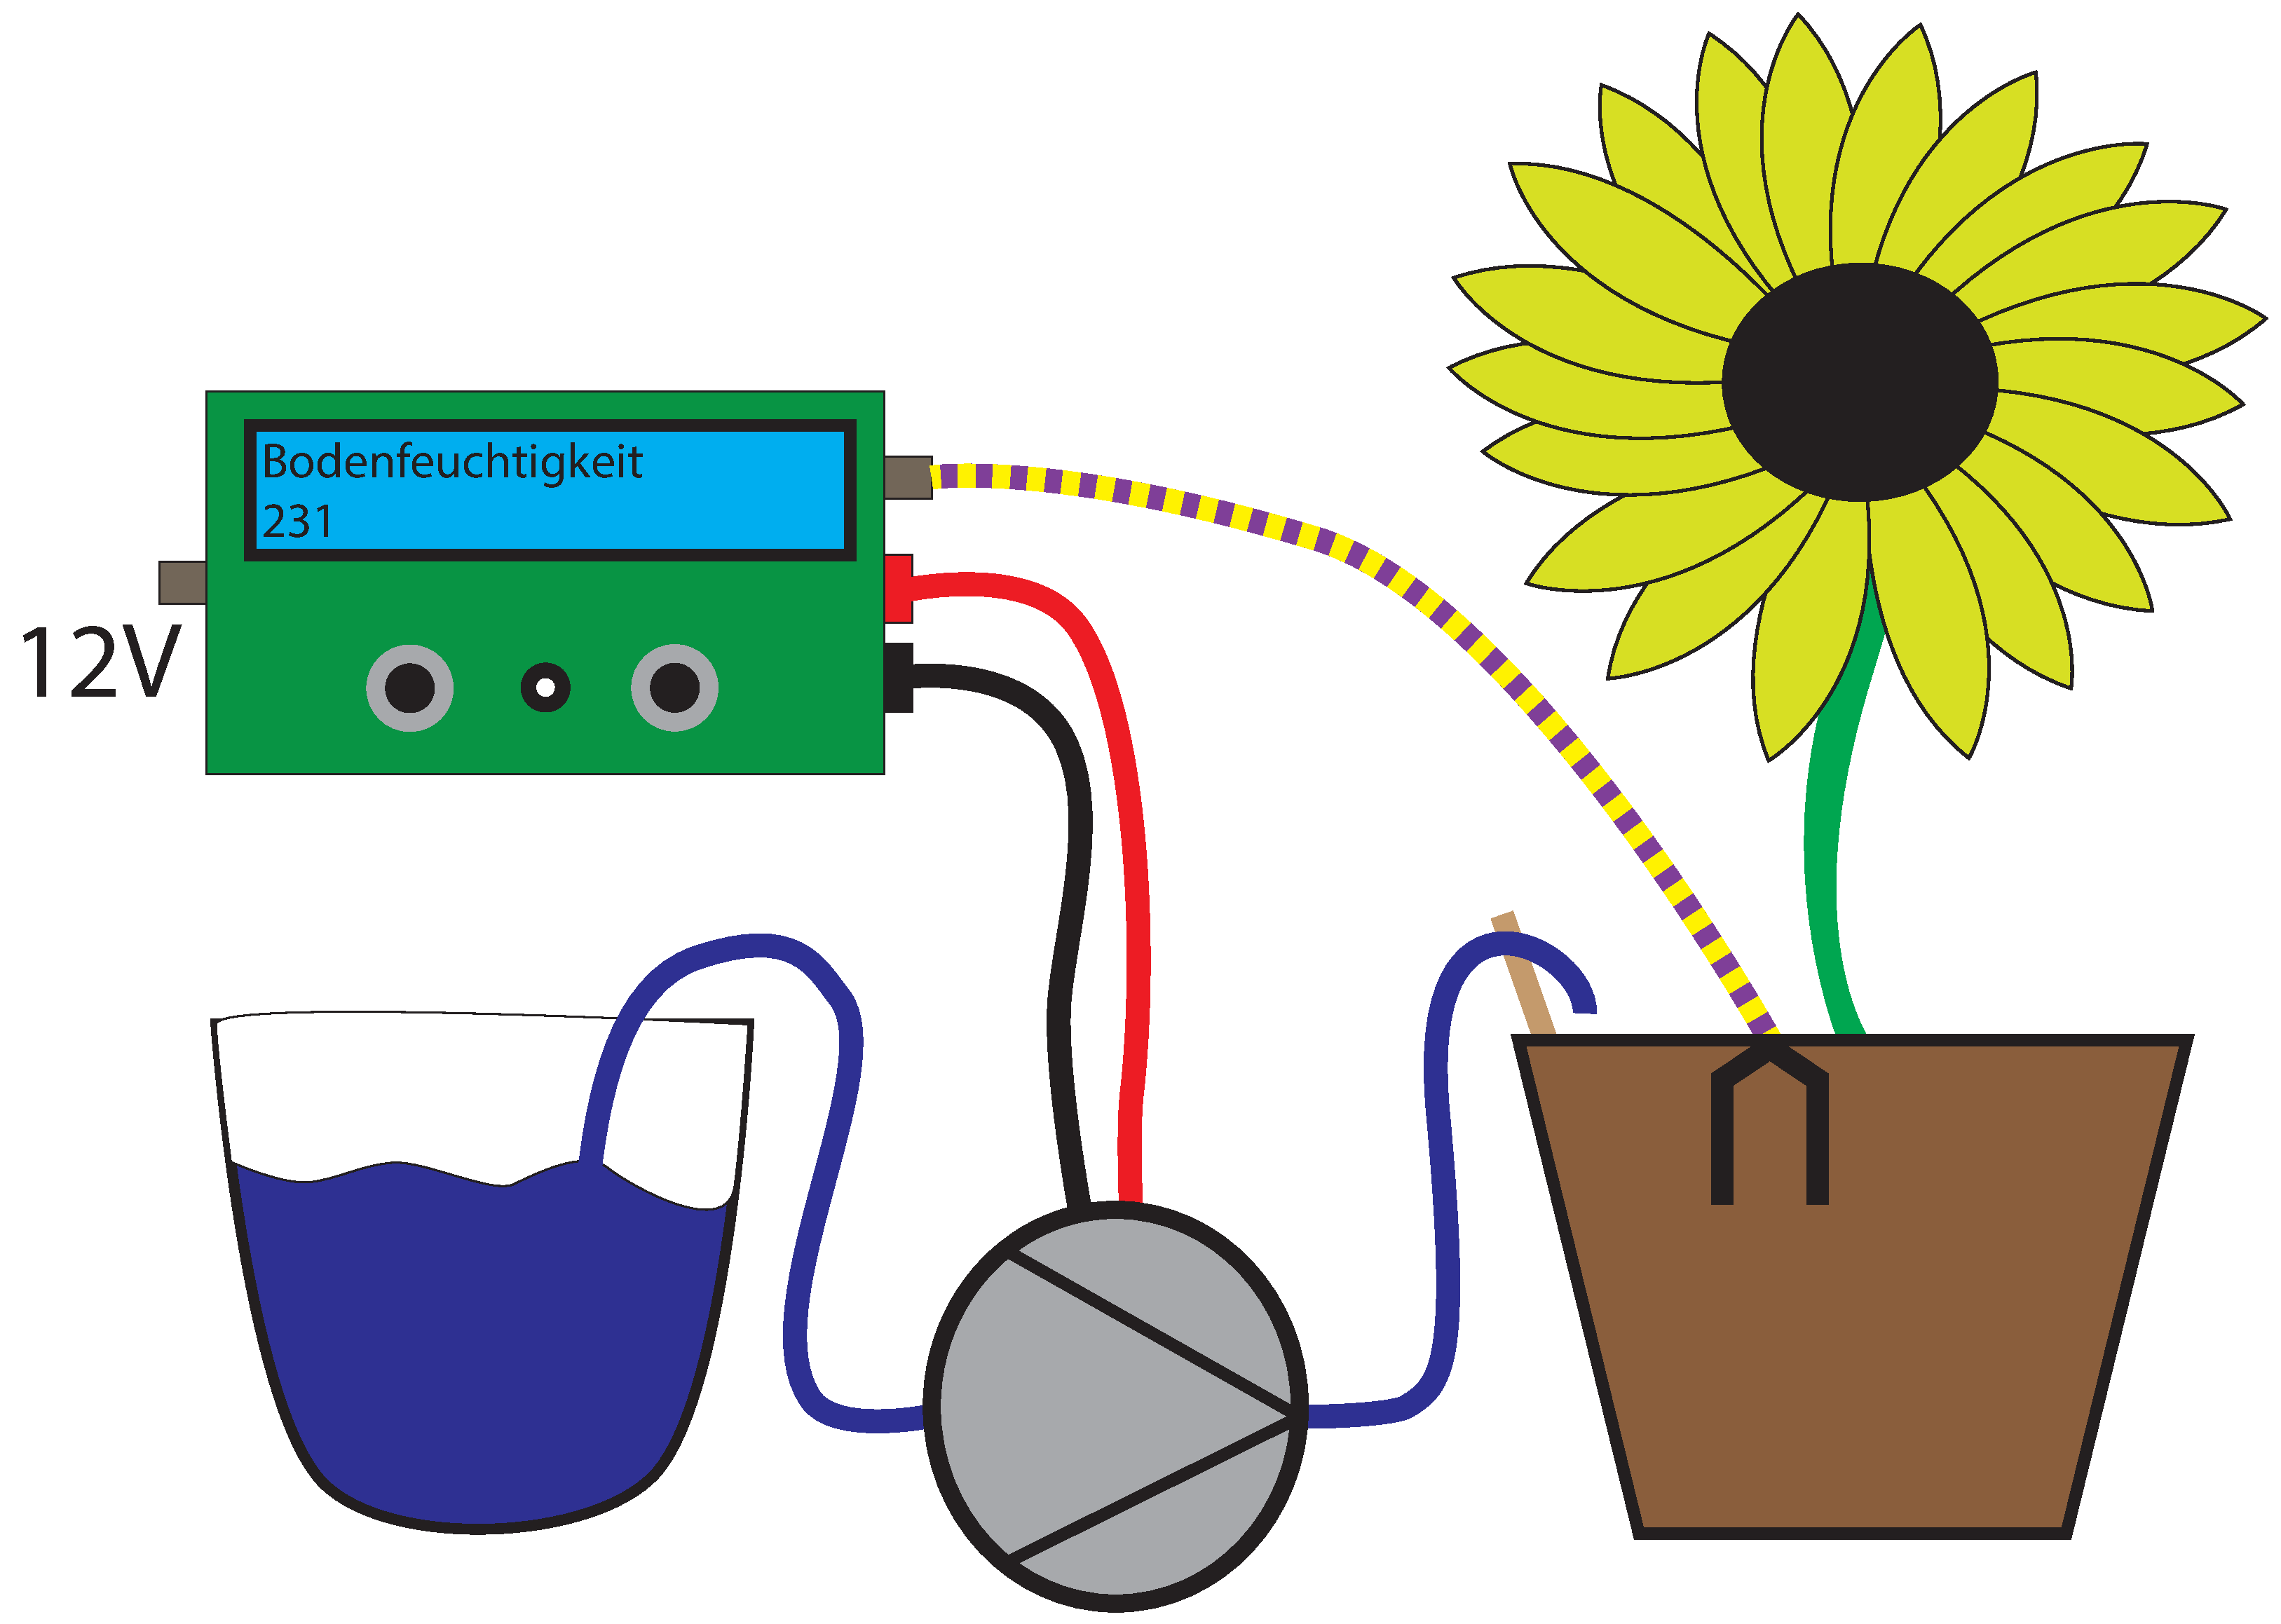
\includegraphics[width=0.8\linewidth]{bilder/Bild_Aufbau.eps}	
	\caption{Schematischer Aufbau der Gießanlage}
	\label{fig-SchemaAufbau}
	\end{figure}

\subsection{Wassertransport}
Um den Einsatzbereich so flexibel wie möglich zu halten haben wir uns für ein Pumpensystem entschieden. 
Dadurch ist die Anordnung der Pflanze zum Wassertank nicht relevant. 
Der hiermit einhergehen erhöhte Strombedarf ist zu verkraften, da unser System nicht auf Batterien angewiesen ist.

Für den Wassertransport haben wir uns für eine Zahnradpumpe entschieden.
Die Zahnradpumpe gehört zu der Gruppe der rotierenden Verdränger Pumpen 
\footnote{\href{http://www.ksb.com/Kreiselpumpenlexikon\_de/Pumpenlexikon/1563382/verdraengerpumpe.html}{www.ksb.com/Kreiselpumpenlexikon\_ \\ de/Pumpenlexikon/1563382/verdraengerpumpe.html}}.
Das Fördermedium wird hierbei zwischen zwei Zahnrädern in einem in sich geschlossenen Volumenbereich gefördert.
Die Bauweise dieser Pumpe ermöglicht zudem einen selbstsaugenden Betrieb. 
Dies bedeutet, dass diese Pumpe in der Lage ist Gase zu transportieren und somit einen Unterdruck in der Zuleitung zu erzeugen, der ausreicht, um das Fördermedium (in unserem Fall Wasser) anzusaugen. 
Diese Eigenschaft war schlussendlich ausschlaggebend, dass sich die Zahnradpumpe gegenüber den anderen Lösungen durchgesetzt hat.
Als Alternativen wurden Ventile und Kreiselpumpen angedacht.
Die Kreiselpumpe konnte trotz dem geringeren Stromverbrauch und geringerem Geräuschpegel nicht durchsetzen. 
Noch weniger Strom und Lärm verursachen Ventile, die aber auf gespeicherte Energie angewiesen sind.  
Entweder durch Druck im Wassertank oder durch Erhöhung des Tankes über den Ausfluss. 
Auf Grund der Wahl der Zahnradpumpe kann ein 4\,mm Schlauch zur Förderung des Wassers genutzt werden, der nahezu beliebig verlegt werden kann.  
Ebenso ist das Gefäß frei wählbar, für das Testsystem haben wir eine 1,5\,Liter Flasche verwendet. Im Dauerbetrieb wird ein fünf-Liter"~Weinballon verwendet. 
In der Pflanze wird der Schlauch mit einem durchbohrten Kantholz in der Pflanzenerde befestigt.

	
\begin{table}
	\centering
		\onehalfspacing
	\footnotesize
	\caption{Vergleich Wasserpumpen und Ventil}
	\label{Vergleich zwischen Wasserpumpen und Ventil}
		\begin{tabular}{|l|lll|}
		\hline
		\textit{Eigenschaft} & \textit{Zahnradpumpe} & \textit{Kreiselpumpe} & \textit{Ventil} \\
		\hline
		Selbstsaugend	&ja	&nein &nein\\		
		Lautstärke		&sehr laut	&mittel laut	&leises Klacken\\
		Stromverbauch	&@12V 2,8A	&@12V 0,6A	&@12V 80mA\\
		Förderleistung	&gering		&groß		&keine eigene\\
		Preis			&2,95 \euro	& 2,95 \euro	&	4,95 \euro\\
		\hline		
		\end{tabular}
		
\end{table}	
	
	
	
\subsection{Gehäuse}
	Das Gehäuse wurde so konzipiert, dass es möglichst klein ist aber genügend Platz für die Elektronik bietet.
	Im Gehäuse verbaut sind:
\begin{itemize}
	\item ein LCD-Display zur Anzeige der Gießparameter (aktelle Feuchtigkeit, Gießintervall \dots)
	\item zwei Taster zur Steuerung der Displayanzeige und zum manuellen Gießen
	\item der Photowiderstand zur Messung der Helligkeit (platziert zwischen den Tastern)
	\item Stromschluss auf der linken Seite
	\item Ausgänge für die Pumpe und den Feuchtigkeitssensor auf der rechten Seite

\end{itemize}	

	\begin{figure}[!h]
	\centering
	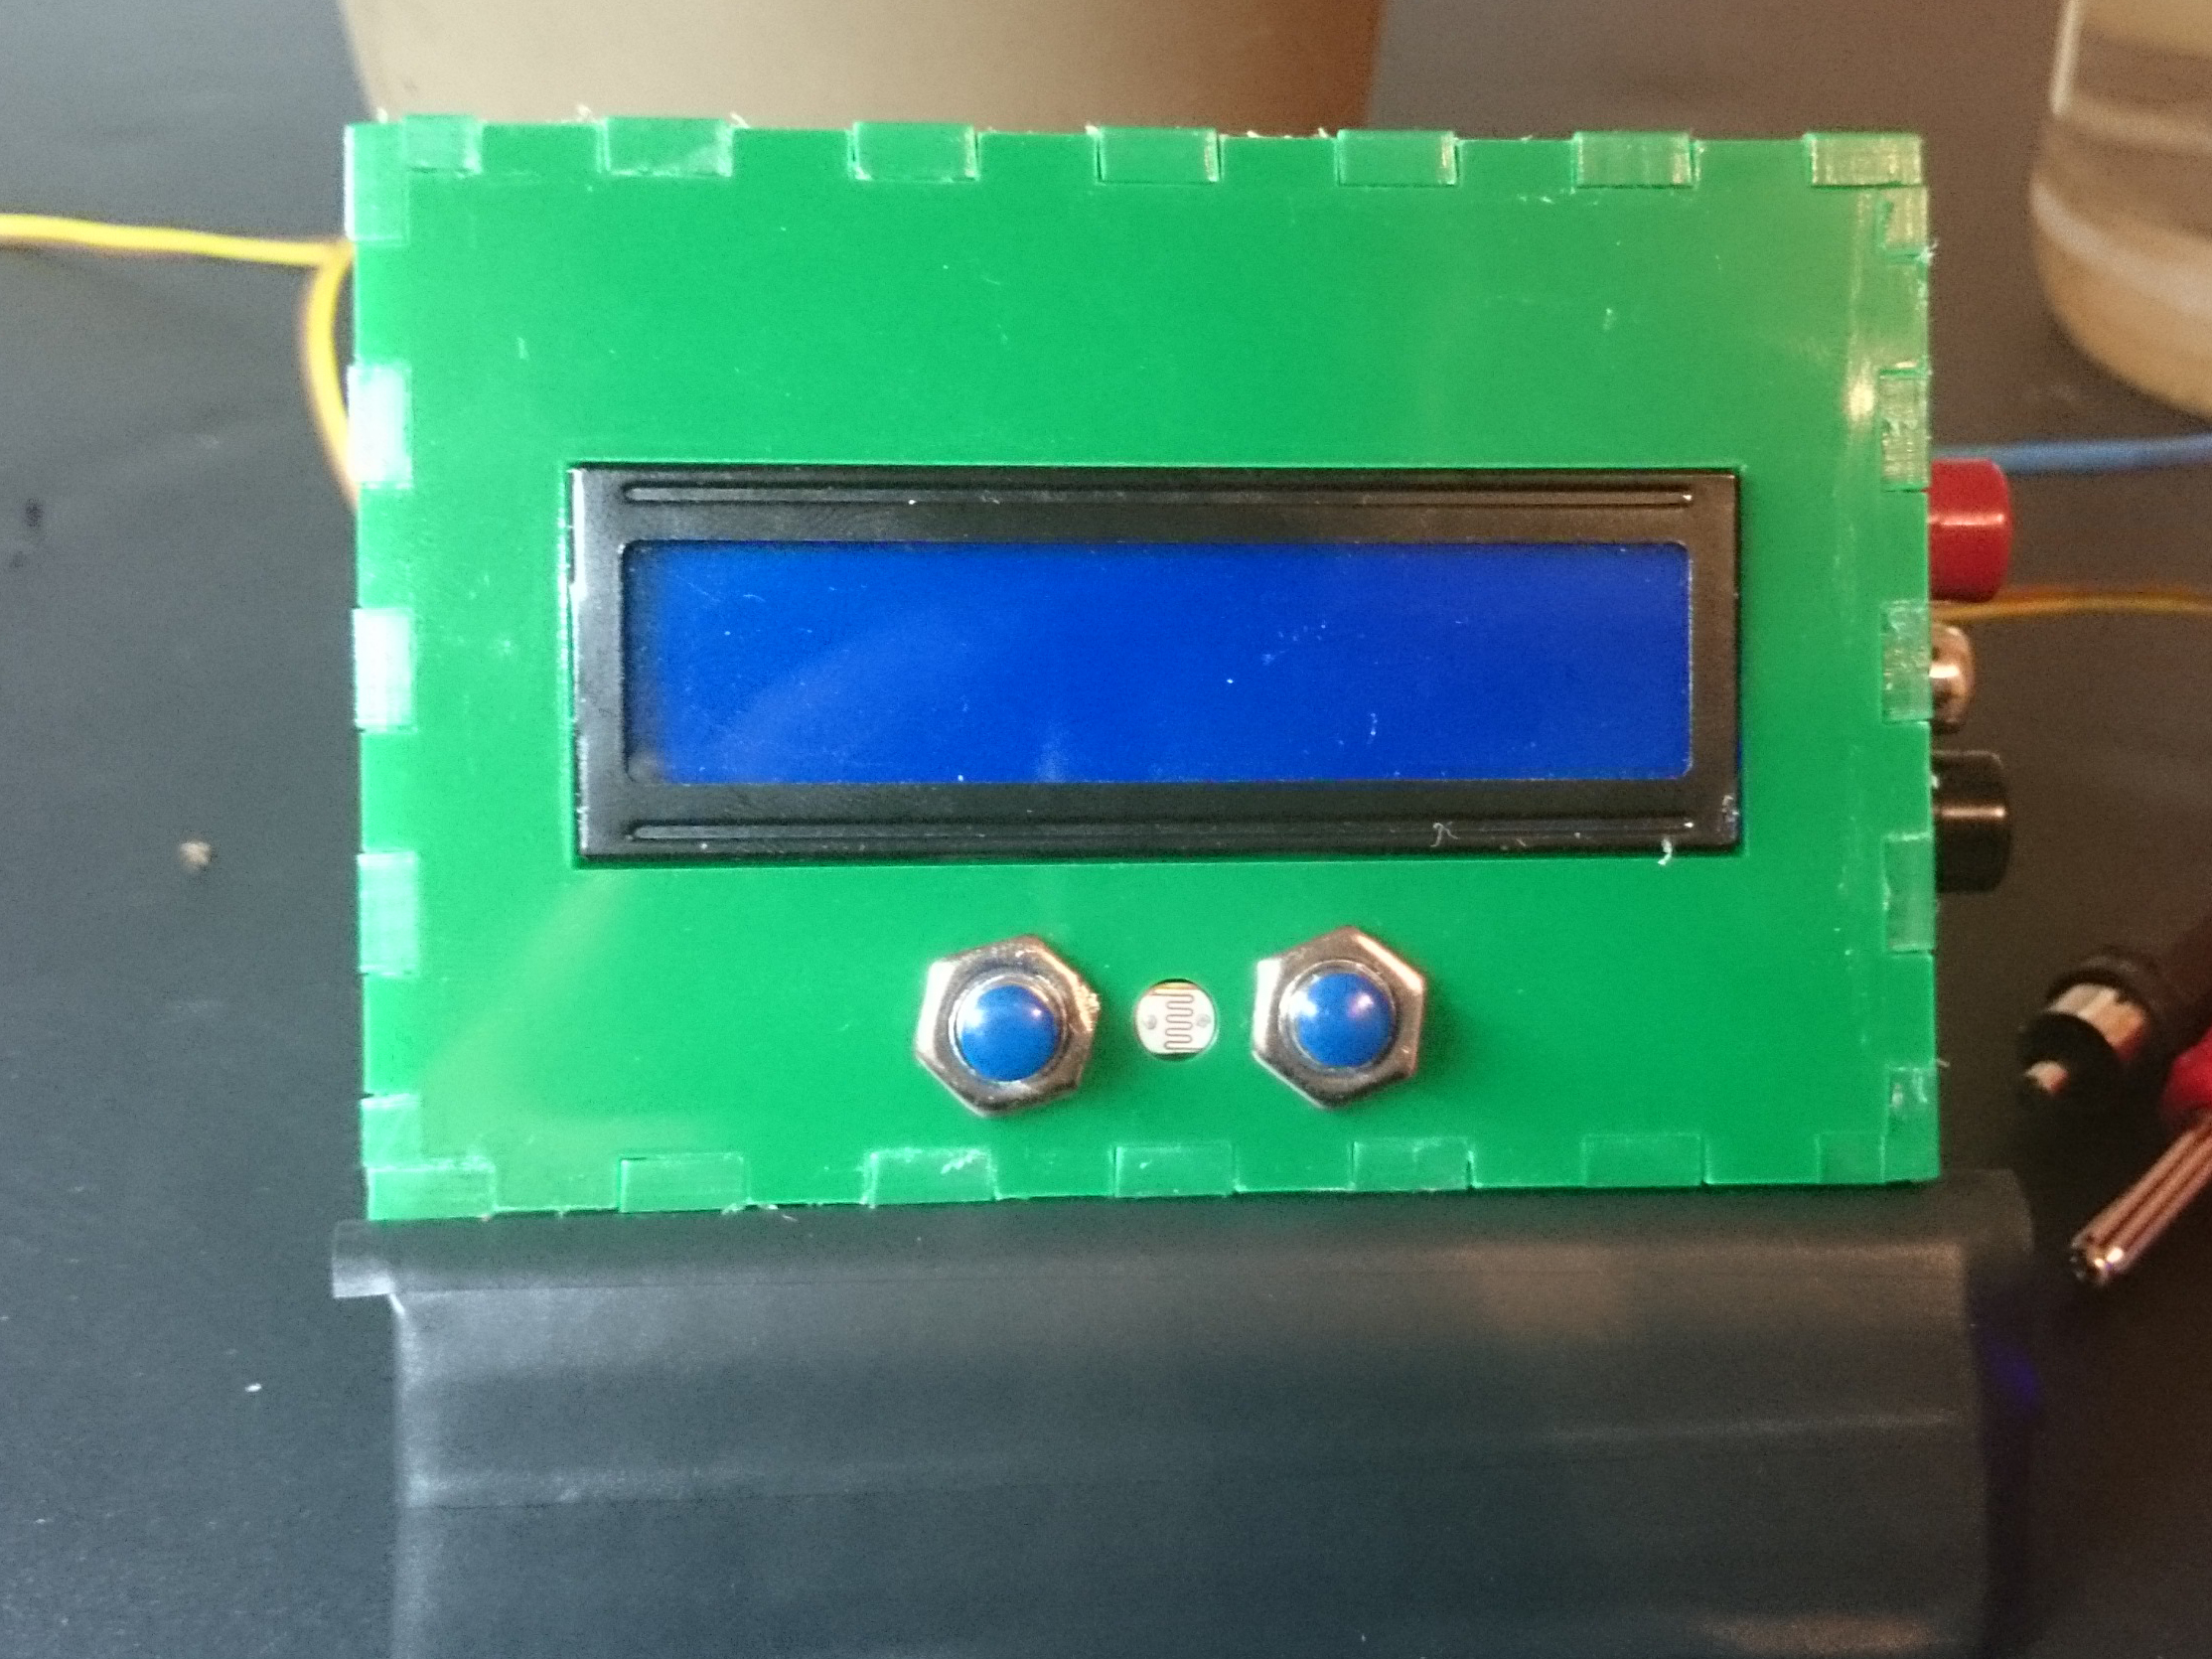
\includegraphics[width=0.8\linewidth]{bilder/_boxFron1.jpg}	
	\caption{Gehäuse Frontansicht}
	\label{fig-Gehäuse}
	\end{figure}
	
Das Gehäuse wurde in FabLab Erlangen mit einem Lasercutter gefertigt. 
Für das Design des Gehäuses wurde der BoxMaker\footnote{ \href{http://boxmaker.connectionlab.org/}{http://boxmaker.connectionlab.org/}} verwendet. 
Das Gehäuse besteht aus grünen 3\,mm dicken Acrylglas.
	
\subsection{Elektronik}
Im folgenden wird der Aufbau der Version~1.0 der Arduino Variante vorgestellt. 
Während des Aufbaus, vor allem aber während der Testphase sind ein paar Probleme aufgetreten die dazu geführt habe, dass eine neue Version~1.1 erstellt werden musste. 
Diese neue Version ist jedoch aus zeitlichen Gründen noch nicht komplett aufgebaut. 
Ein neues Layout wurden bereits erstellt und die Software ist so angepasst worden, dass diese ohne größere Änderungen übernommen werden kann. 
Daher wird im folgenden die Funktionsweise auf Basis der Version~1.0 erläutert, an gegebener Stelle wird auf die Anpassungen eingegangen, die bereits umgesetzt wurden bzw. noch in Planung sind. 

			
\subsubsection{Sensorik} \label{sensorik}
Für den Helligkeitssensor wird ein einfacher Photowiderstand verwendet, der über einen Spannungsteiler an einem der Analogen Pins des Arduino Bords angeschlossen ist. Der Pin verfügt über einen 10\,Bit AD Konverter und gibt demnach einen Integerwert von 
0\,-\,1023 zurück.
Der Bodenfeuchtigkeitssensor bestimmt den Wassergehalt des Bodens über eine Widerstandsmessung zwischen den zwei Zinken einer Messgabel. 
Je mehr Wasser im Erdreich vorhanden ist, desto kleiner ist der gemessene Widerstand im Boden.

\begin{figure}[!h]
	\centering
	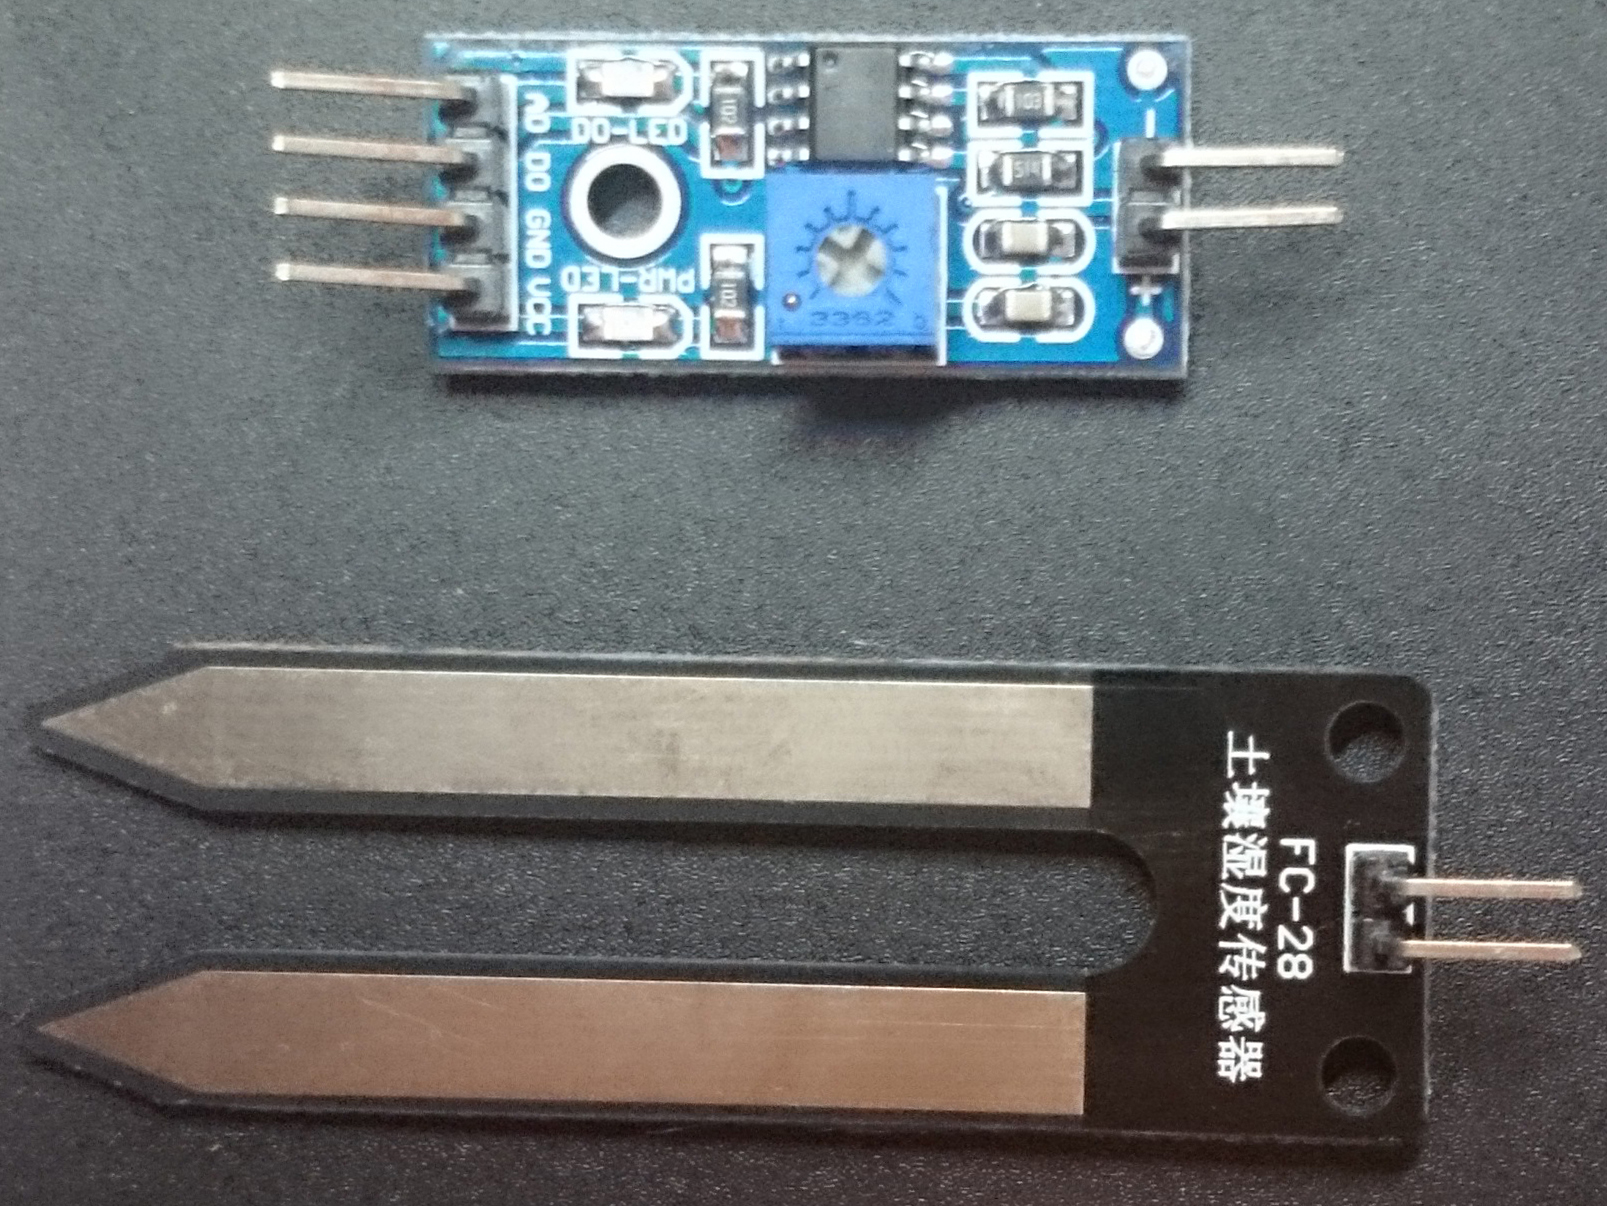
\includegraphics[width=0.8\linewidth]{bilder/_feuchteSensor1.jpg}
	\caption{Feuchtigkeitssensor mit Vorschaltung}
	\label{fig-SensorVorschaltung}
\end{figure}
Der Feuchtigkeitssensor benötigt keine weiteren Schaltelemente, da er über eine eine Vorschaltung verfügt in der ein Spannungsteiler bereits verbaut ist. 
Abbildung \ref{fig-SensorVorschaltung} zeigt den verwendeten Sensor und die Vorschaltung. 
Es ist möglich sowohl den Analogen Wert, oder ein Digitales Signal auszuwerten. 
Das Digitale Signal liefert einen Null"-wert solange ein Grenzwiderstand nicht überschritten wird. 
Über ein  Potentiometer(siehe Abbildung \ref{fig-SensorVorschaltung}) lässt sich diese Grenze einstellen. 
Wegen des schlechten Zugangs zum Potentiometer im eingebautem Zustand wird der Digitale Output nicht verwendet, sondern der Analoge Messwert selbst ausgewertet und mit einer Variablen im Mikrocontroller abgeglichen.
		
\emph{Anpassung zu Version~1.1:}
Leider zeigte sich, dass nach nur 48 Stunden Dauermessung die Gabel erhebliche Korrosion erlitten hat, Abbildung \ref{fig-SensorVergleich} zeigt dies deutlich.
Die Vorschaltung sieht keine Abschaltung des Messprozesses vor noch eine Umpolung der Gabel. 
Deswegen muss die gesamte Vorschaltung stromlos geschaltet werden, um das Auflösen des Sensors zu verlangsamen. 
Hierfür haben, wir für die Version~1.1, eine Transistorschaltung für den Sensor eingefügt. 
Über diese Schaltung wird die Vorschaltung des Feuchtigkeitssensor stromlos geschaltet und der Sensor ist nur für eine Messung unter Strom. 
Eine Umpollung der Messgabel ist auch nicht möglich, dies kann jedoch relativ einfach dadurch gelöst werden, indem der Sensor alle paar Wochen \emph{manuell} umgepolt wird. 
Hierfür muss lediglich die Messgabel vom Verbindungskabel abgesteckt werden und um \begin{math}180^{\circ}\end{math} gedreht wieder verbunden werden.

\begin{figure}[!h]
	\centering
	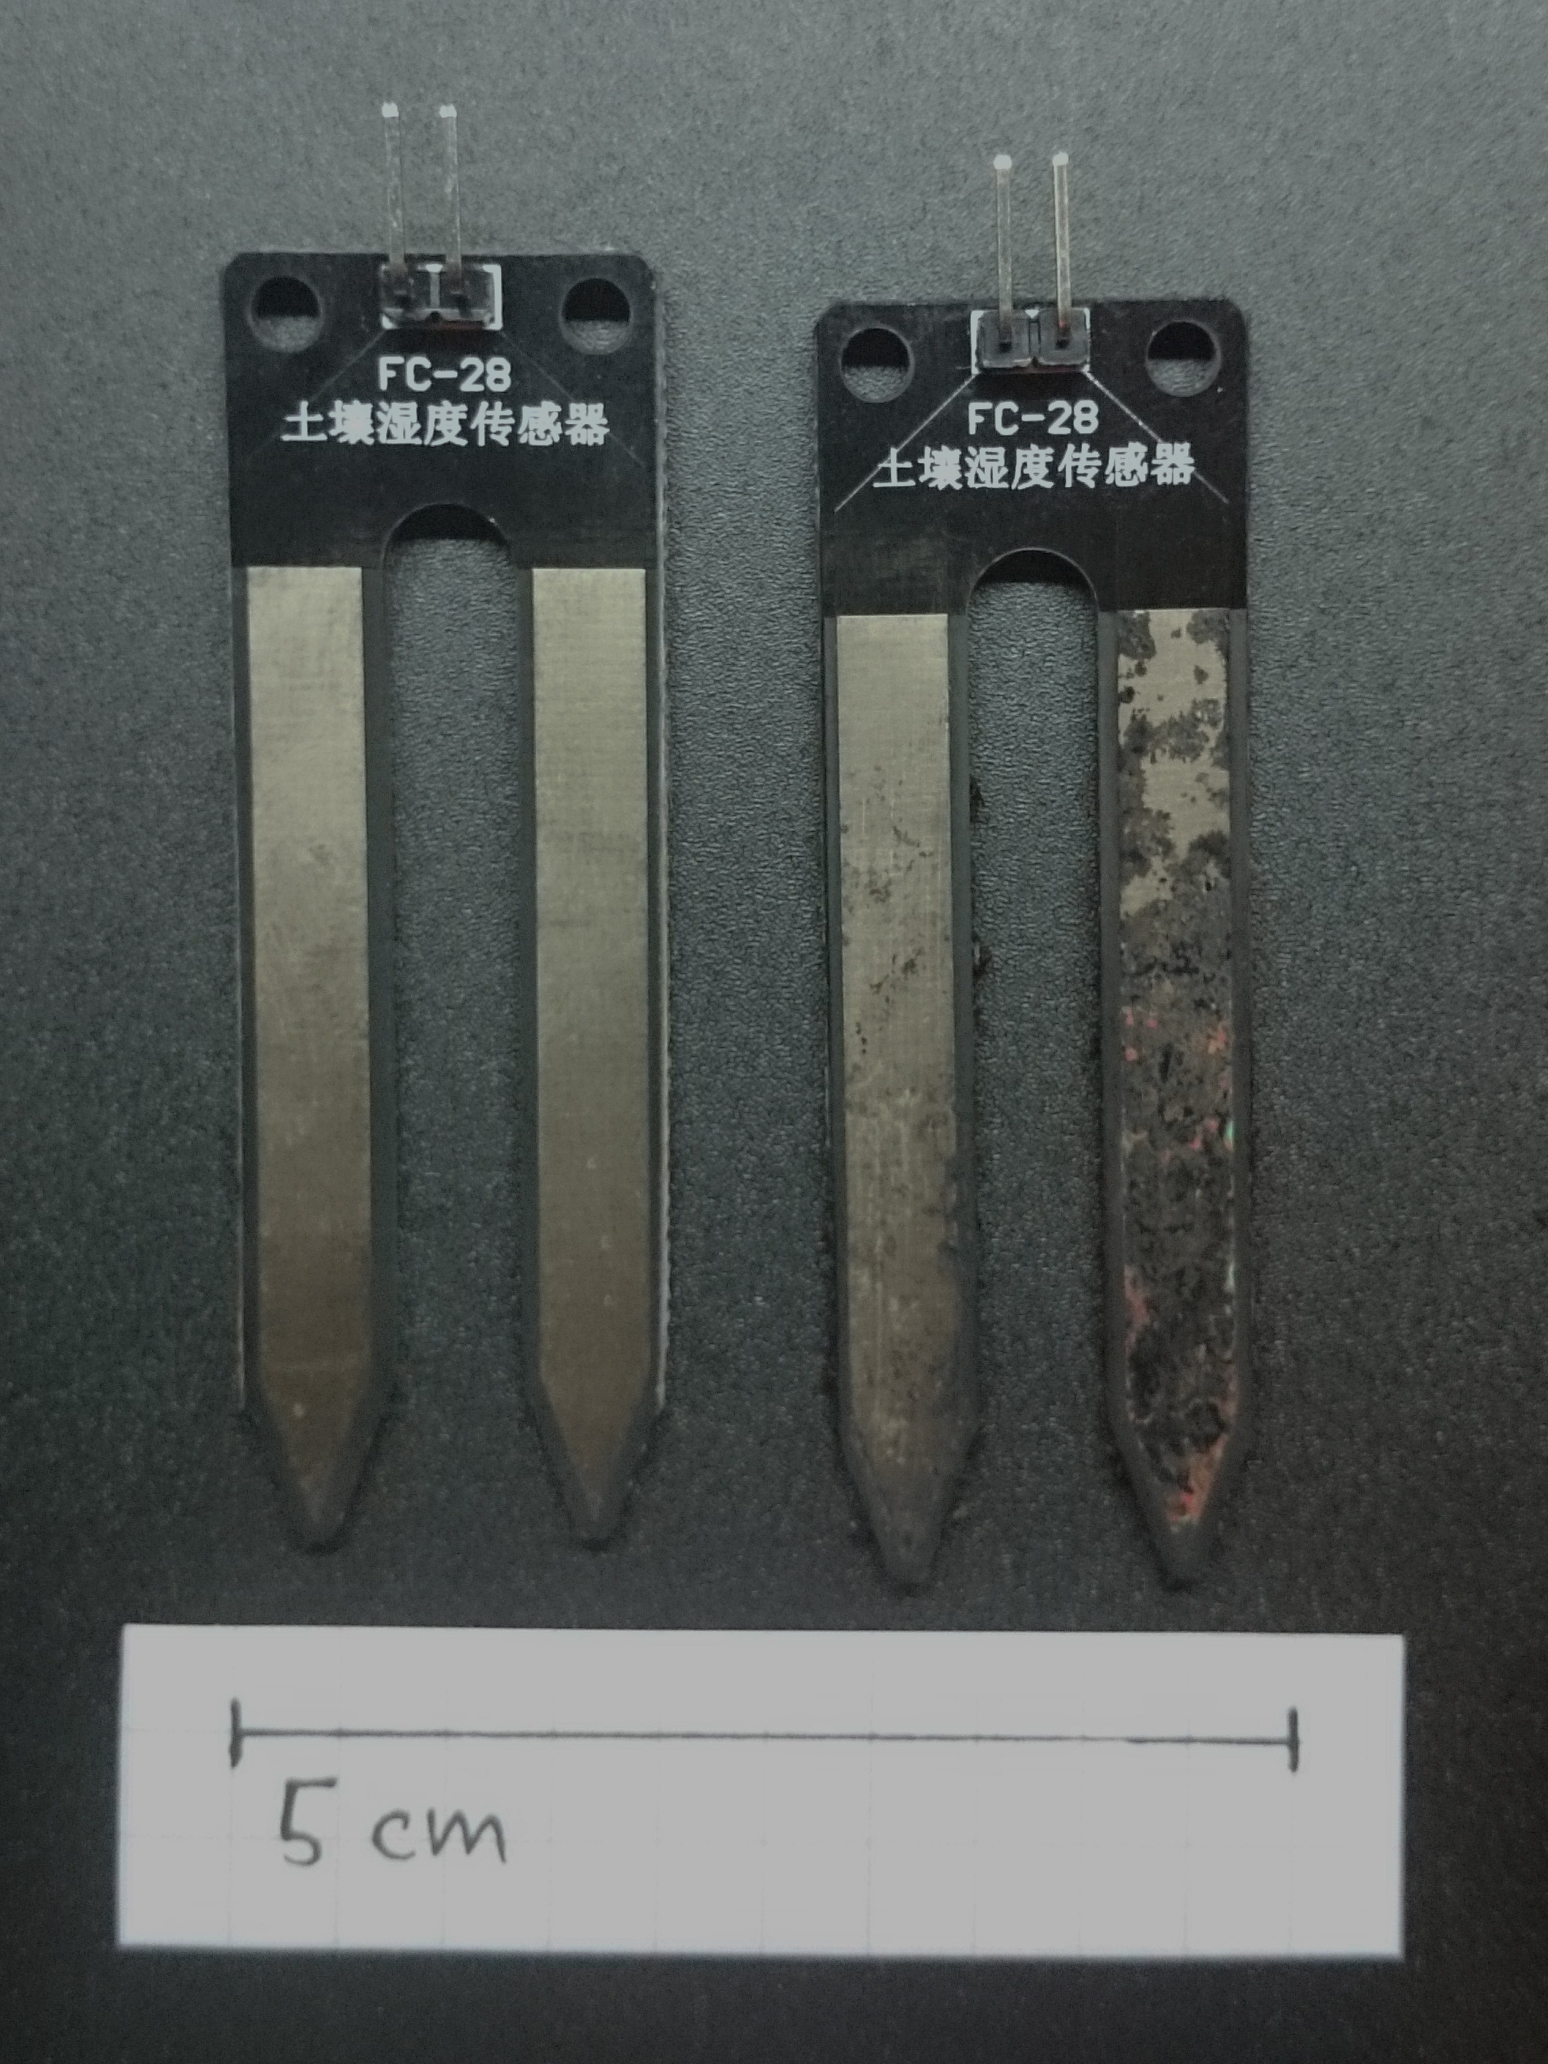
\includegraphics[width=0.8\linewidth]{bilder/_fechtesensorVergleich0.jpg}
	\caption{Vergleich neuer Sensor und Sernsor mit 48h Dauerbetrieb}
	\label{fig-SensorVergleich}
\end{figure}

\subsubsection{Kommunikation}
Jede Pflanze braucht unterschiedlich viel Wasser. 
Genauso hat die Zusammensetzung der Erde einen Einfluss auf den gemessenen Widerstand des Feuchtigkeitssensors.
Ziel der Kommunikation soll es deswegen sein, dass Gießsystem im laufenden Betrieb zu kalibrieren. 
Wir haben uns für eine drahtlose Kommunikation, auf Basis des XBee Standard, entschieden. 
Das XBee Modul wurde direkt, d.h. ohne Verwendung eines \emph{Arduino XBEE"~Shields}, mit dem Arduino verbunden. 
Hierfür ist es notwendig einen Pegelwandlung von 5\,V auf 3,3\,V vorzunehmen, da die Logik-Pins des XBee Moduls nicht mit 5\,V betrieben werden können. 
%%%%%%
Abbildung \ref{fig-Pegel} zeigt die Umsetzung der Pegelschaltung. Die Lables \emph{TXD} und \emph{RXD} repräsentieren die jeweiligen Anschlüsse am Arduino Micro. In dieser Schaltung lassen sich drei Zustände erkennen\footnote{http://www.adafruit.com/datasheets/an97055.pdf; Seite 10f}
\begin{itemize}
\item Wird keiner der beiden Seiten (Mikrocontroller bzw. XBee) auf GND gezogen, so werden die Eingänge durch ihre  Pull-Up 	Widerstände auf 5\,V bzw. 3,3\,V gezogen. Dadurch ist das Spannungsgefälle \emph{Gate"~zu"~Source} gleich Null, da an beiden 	Anschlüssen 3,3\,V anliegen. Der Transistor ist nicht leitend.
\item Wird am XBee (DOUT) ein LOW Signal angelegt, so steigt das Spannungsfälle \emph{Gate"~zu"~Source} an und der Transistor wird leitfähig, was dazu führt das auch die Pins am Mikrocontroller(RXD) auf LOW gezogen werden.
\item Wird hingen auf der Seite des Mikrocontroller (TXD) ein LOW Signal angelegt, so wird über die die Diode im Transistor das Spannungspotenzial der Source solange reduziert, bis das Spannungsgefälle \emph{Gate"~zu"~Source} groß genug wird, damit der Transistor leitfähig wird. Sobald dieser Grenzwert überschritten wird, wird auch DOUT am Xbee auf LOW gezogen.
\end{itemize}

Bei der Pegelschaltung ist uns in Version~1.0 ein Fehler unterlaufen, weswegen wir keine Verbindung mit ein Computer aufbauen konnten. Dieser Fehler ist für die Version~1.1 behoben.

\begin{figure}
	\centering
	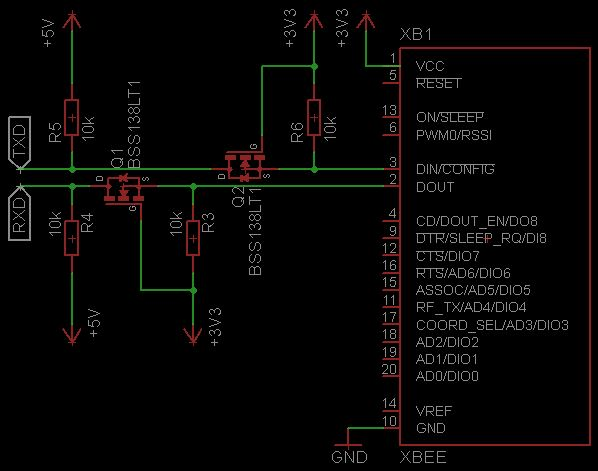
\includegraphics[width=0.8\linewidth]{bilder/v1SchaltplanXbee.jpg}
	\caption{Pegelwandler mit Small-Signal-Transistor BSS138W }
	\label{fig-Pegel}
\end{figure}
		
Die zweite Schnittstelle mit dem Menschen wird über ein Display ermöglicht. 
Hier lässt sich über einen Taster die einzelnen Variablen mit ihren aktuellen Werten Überprüfen. 
Bei dem Display Handelt es sich um ein 2 Zeiliges LCD"~Display mit jeweils 16 Zeichen. 
Die Kommunikation zwischen Display und Mikrocontroller wird über eine I2C"~Schnittstelle bewerkstelligt. 
Hierfür haben wir die frei verfügbare \mbox{LiquidCrystal\_I2C} Libary von fderbrabander verwendet.\footnote{\href{https://github.com/fdebrabander/Arduino-LiquidCrystal-I2C-library}{https://github.com/fdebrabander/Arduino-LiquidCrystal-I2C-library}}

\begin{figure*}[!h]
	\centering
	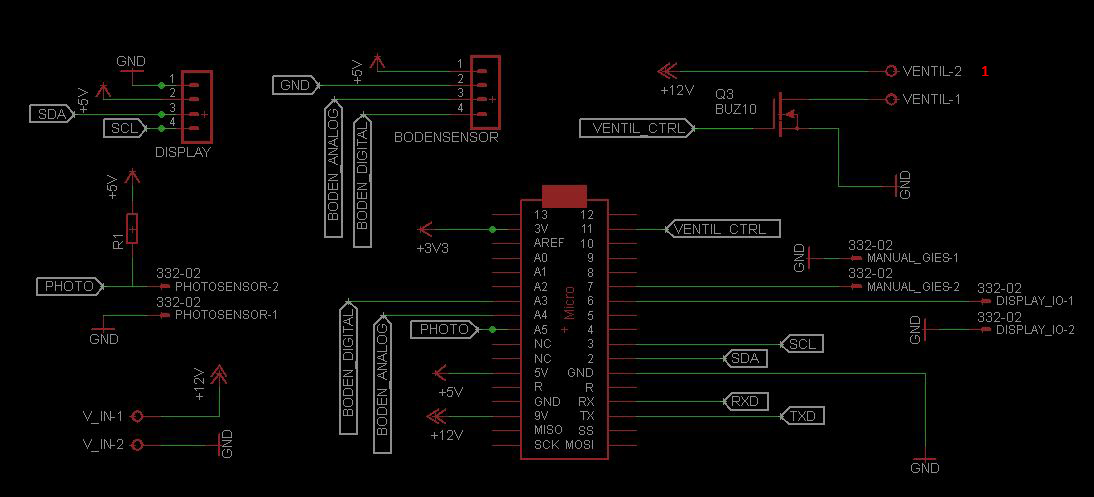
\includegraphics[width=0.9\linewidth]{bilder/v1SchaltplanMicro0.JPG}
	\caption{Schaltpaln V1.0 mit Arduino Micro}
	\label{fig-Schaltplanv1.0}
\end{figure*}

	
\subsubsection{Stromversorgung}

Eine Stromversorgung über USB ist nicht möglich, da die Pumpe in Voll"-last 12\,V und außerdem 2,8\,A benötigt. 
Deswegen muss auf eine leistungsfähigere Energiequelle gesetzt werden.
Wir entschieden uns für Netzteile mit 12\,V Ausgangs"-spannung um die Pumpe direkt anschließen zu können. 
Um den Strom der Pumpe zu begrenzen haben wir einen \begin{math}5~\Omega\end{math} Lastwiderstand in Reihe geschaltet.
Dies führt zu geringerer Leistungsaufnahme und deutlichen Geräusch"-minderung.
Die Ansteuerung der Pumpe über dem Mikrocontroller ist über eine Transistorschaltung gelöst (Ziffer 1 in Abbildung \ref{fig-Schaltplanv1.0}).
Es ist zu überlegen, den Transistor und den Mikrocontroller über eine Schutzdiode über die Anschlüsse \emph{VENTIL-1} und \emph{VENTIL-2} vor Überspannung zu schützen, die beim Abschalten der Pumpe auftreten können. 
 

\subsection{Programm}
	

	Die Aufgaben des Mikrocontrollers sind die folgenden:
		\begin{itemize}
			\item Messung der Feuchtigkeit
			\item Messung der Helligkeitssensor
			\item Vergleich der Messwerte mit den festgelegten Grenzen
			\item Ansteuerung der Pumpensystem
			\item Ausgabe der wichtigen Variablen auf dem Display über Taster
			\item Manuelles Gießen über Taster
			\item Display Hintergrundbeleuchtung abschalten nach 60  Sekunden
			\item Übertragen/Empfangen von Einstellungen über xBee Verbindung
		\end{itemize}
		
	In der ersten Version wurden die Messungen andauernd durchgeführt. 
	Wie aber bereits oben erläutert hat dies zu einer starken Korrosion am Feuchtigkeitssensor geführt. 
	Aus diesem Grund wurde für die Version~1.1 einige Änderungen eingeführt. 
	Anstelle bei jedem Aufruf der Loop() Methode eine Messung durchzuführen wird nur noch alle 4 Stunden eine Messung vorgenommen. 
	Ist das Intervall abgelaufen wird der Feuchtigkeitssensor über eine Transistorschaltung angeschaltet und anschließend ausgelesen. 
	Dadurch ist der Sensoren nur noch für einen kurzen Zeitraum unter Strom, was die Lebensdauer des Feuchtigkeitssensor verlängert.
		
	
	%\subsection{Setuptool}
	Da die Erde in jeder Pflanze eine andere Zusammensetzung hat und jede Pflanze unterschiedlich viel Wasser benötigt ist es notwendig die Grenzwerte für die Feuchtigkeit und die Wassermenge einzustellen. 
	Hierfür gibt es ein Cmd-Tool welches über die 
	

	
%\subsection{BOM - Bill of Matirial}
	
\subsection{Kostenplan}
 Durch die geringen Kosten pro Entwicklungsstufe hatten wir genügend Geld um mehrere Iterationsstufen  zu durchlaufen.
 Deswegen benötigten wir für die gesamte Entwicklung etwas über hundert Euro.
 Ein einzelnes Modul kann für etwa 45\,\euro\ nachgebaut werden. 
 Die Kosten setzen sich nach Tabelle\,\ref{Kosten für eine Giessanlage} zusammen.
 
 Nicht berücksichtigt sind das Wassergefäß, die zwei \begin{math}4mm\end{math}\,-Schlauch"-stücke und Befestigung in der Pflanze.
 Bei diesen handelt es sich um Reste oder Lagerfunde die von Wert von unter 1\,\euro\ sind. 
 
\begin{table}[h]
	\centering
	\onehalfspacing
	\footnotesize
	\caption{Kosten für eine Gießanlage}
	\label{Kosten für eine Giessanlage}
		\begin{tabular}{|l|ll|}
			\hline
\textit{Bauteil} & \textit{Kosten} & \textit{Bezugsquelle} \\
\hline
Arduino Nachbau & ca. 3 \euro & ebay \\
LCD-Display & ca. 5 \euro & ebay\\
Bodensensoren & ca. 2 \euro & ebay \\
Zahnradpumpe & 2,95 \euro & Pollin \\
XBee &  23,55 \euro & Reichelt \\
Hauptplatine & ca. 6 \euro & FabLAB \\
Gehäuse	& ca. 4 \euro & FabLAB \\

\hline
Gesamt: & ca 45 \euro & \\
\hline
\end{tabular}
\end{table}
